\section{Hyperparameters}\label{sec:hyperparams}

In the previous section on regularization we introduced the regularization strength $\lambda$ without much fanfare. However that innocuous seeming inclusion has quite far reaching consequences. All of which stem from the question of how do we determine the value of the parameter $\lambda$? There is no analytical solution for the optimal value and so we're left with other ways of estimating its value. As models grow more complex several of these parameters which influence optimization but are not model parameters need to be added; they're collectively known as hyperparameters.

Hyperparameters are parameters in the model that have to be heuristically determined that may impact performance without having a closed form derivative with respect to the optimization problem. These parameters have proven to be vitally important to the optimization of machine learning models. In the simple linear or logistic regression case the hyperparameters include the choice of regularization norm (ordinarily the $L_1$ or $L_2$ norms) and the regularization strength $\lambda$. The choices of all these parameters are highly non-trivial because their relationship can be strongly co- or contra-variant. Additionally the search for these parameters are expensive because each configuration of parameters is accompanied by a full training of the model. In this section we'll discuss the general process of tuning hyperparameters in general, and then we'll introduce specific parameters that need tuning in subsequent sections pertaining to particular architectures or modeling choices. Whichever scheme is chosen for the optimization they each follow the same basic procedure:

\begin{enumerate}
\item Choose hyperparameter configuration
\item Train model
\item Evaluate performance
\item Log performance and configuration
\end{enumerate}

\noindent When searching for hyperparameter configurations for a given model it becomes necessary to define a scale for the variable. Together with the range the scale defines the interval on which we do the search. That is the scale defines the interval width on the range of the parameter. Usually the scale is either linear or logarithmic, though some exceptions exist. As they are discussed for each model type or neural network cell type a suggested scale will also be discussed.

\subsection{Hand holding}
The most naive way of doing hyperparameter optimization is to manually tune the values by observing changes in performance metrics. Being naive and unfounded it is rarely used in modern modeling pipelines, outside the prototyping phase. For this thesis we use a hand held approach to get a rough understanding of the ranges of values over which to apply a more well reasoned approach. 

\subsection{Grid Search}
Second on the ladder of naiveté is the exhaustive search of hyperparameter configurations. This in this paradigm one defines a multi dimensional grid of parameters that is evaluated. If one has a set of $N$ magnitudes of the individual parameter sets $s = \{n_i\}_{i=0}^{N}$ with values of the individual parameters $\gamma_k$ and where $n_i = |\{\gamma_k\}|$ then the complexity of this search is $\mathcal{O}(\prod_{n \in s} n)$. For example in a linear regression we would want to find the optimal value for the learning rate $\eta = \{\eta_k\}$ and the regularization strength $\lambda = \{\lambda_k\}$ then this search is a double loop as illustrated in algorithm \ref{algo:gridsearch}. In practice however the grid search is rarely used as the computational complexity scales exponentially with the number and resolution of the parameters. The nested nature of the for loops is also extremely inefficient in the event that the hyperparameters are disconnected i.e. neither co- or contra-variant.  

\begin{algorithm}[H]
\SetAlgoLined
\KwData{Arrays of float values $\lambda$, $\eta$}
\KwResult{log of performance for each training}
Initialization ;\\
log $\leftarrow [\hspace{0.1in}]$;\\
\For{$\lambda_k \in \lambda$}{
	\For{$\eta_k \in \eta$}{
		opt $\leftarrow$ optimizer($ \eta _k $);\\
		model\_instance $\leftarrow$ model($\lambda _k$);\\
		metrics $\leftarrow$ model\_instance.fit($\mathbf{X}, \mathbf{\hat{y}}$, opt) ;\\
		log.append((metrics, ($\lambda_k$, $\eta_k$)))
	}
}
\caption{Showing a grid search hyperparameter optimization for two hyperparameters $\eta$ and $\lambda$}\label{algo:gridsearch}
\end{algorithm}

\subsection{Random Search}
Surprisingly the hyperparameter search method that has proven to be among the most effective is a simple random search. \citet{Bergstra2012} showed empirically the inefficiency of doing grid search and proposed the simple remedy of doing randomized configurations of hyperparameters. The central argument of the paper is elegantly presented in figure \ref{fig:randomsearch}. Observing that grid search is both more computationally expensive and has significant shortcomings for complex modalities in the loss functions we approach the majority of hyperparameter searches in this thesis by way of random searches. The algorithm for the random search is  very simple in that it just requires one to draw a configuration of hyperparameters and run a fitting procedure $N$ times and log the result. In terms of performance both grid and random search can be parallelized with linear speedups. 

\begin{figure}[H]
\centering
\hspace*{-1.3in}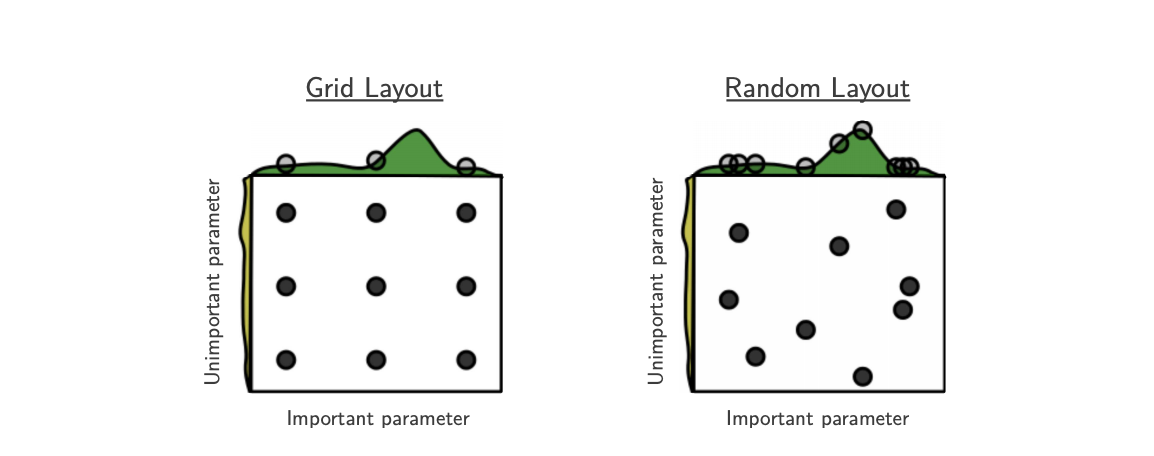
\includegraphics{../figures/randomsearch.png}
\caption[Why randomsearch works]{Figure showing the inefficiency of grid search. The shaded areas on the axis represent the unknown variation of the cost as a function of that axis-parameter. Since the optimum of the loss with respect to a hyperparameter might be very narrowly peaked a grid search might miss the optimum in it's entirety. A random search is less likely to make the same error as shown by \citet{Bergstra2012}. Figure copied from \citet{Bergstra2012}}\label{fig:randomsearch}
\end{figure} 
